\documentclass{book}
\usepackage{ctex}
\usepackage{xcolor}
\usepackage{hyperref}
\usepackage{graphics}

\title{\Large Git tutorial }

\author{LeeMoo}


\begin{document}

\maketitle
\tableofcontents
\subsection{}
The entire pro Git book, written by Scott Chacon and Ben Straub and published by Apress, is availble here. All conteent is licensed under the Creative Commons Attribution Non Commericial Share Alike 3.0 license. Print versions of the book are available on \href{www.amazon.com}{Amazon.com}.\\

\chapter{起步}
	\section{关于版本控制}
	\subsection{关于版本控制}
	\paragraph{}
	什么是版本控制?我为什么要关心它呢?版本控制是一种记录一个或若干个文件内容变化,以便将来查阅特定版本修订情况的系统。在配中所展示的例子中,我们仅对保存着软件源代码的广西文件作版本控制管理,但实际上,你可以对任何类型的文件进行版本控制。\\
	如果你是位图形或网页设计师,可能会需要保存某一幅图片或页面布局文件的所有修订版本(这或许是你非常渴望拥有的功能)。采用版本控制系统(VCS)是个明智的选择。有了它你就可以将某个文件回溯到之前的状态,你可以比较文件的变化细节,查出最后是谁修改了哪个地方,从而找出导致怪异问题的原因,又是谁在何时报告了某个功能缺陷等等.使用版本控制系统通常是意味着,就算你乱来一气把整个项目的文件改的改删的删,你也照样可以轻松恢复到原先的样子.但额外增加的工作量却微乎其微。\\
	\subsection{本地版本控制系统}
	\paragraph{}
许多人习惯用复制整个项目目录的方式来保存不同的版本,或许还会改名加上备份的时间以示区别.这么做唯一的好处就是简单.不过坏处也不少:有时候会混淆所在的工作目录,一旦弄错文件丢了数据就没法撤销恢复.\\
	为了解决这个问题,人们很久以前就开发了许多种本地版本控制系统,大多都是采用某种简单的数据库来记录文件的历次更新差异(如图1-1)。\vfill
	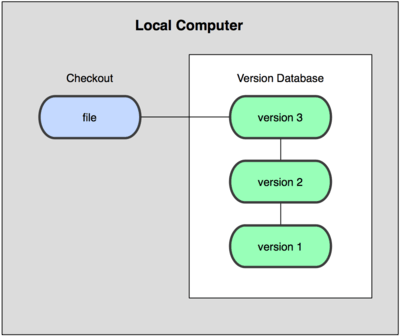
\includegraphics{1-1.png}

	\section{Git简史}
	\section{Git基础}
	\section{安装Git}
	\section{初次运行Git前的配置}
	\section{获取帮助}
	\section{小结}

\chapter{Git基础}
	\section{取得项目的Git仓库}
	\section{记录每次更新到仓库}
	\section{查看提交历史}
	\section{撤消操作}
	\section{远程仓库的使用}
	\section{打标签}
	\section{技巧和窍门}
	\section{小结}

\chapter{Git分支}

	\section{何谓分支}
	\section{分支的新建与合并}
	\section{分支的管理}
	\section{利用分支进行开发的工作流程}
	\section{远程分支}
	\section{分支的衍合}
	\section{小结}

\chapter{服务器上的Git}
	\section{协议}
	\section{在服务器上部署Git}
	\section{生成SSH公钥}
	\section{架设服务器}
	\section{公共访问}
	\section{GitWeb}
	\section{Gitosis}
	\section{Gitolite}
	\section{Git守护进程}
	\section{Git托管服务}
	\section{小结}

\chapter{分布式Git}
	\section{分布式工作流程}
	\section{为项目作贡献}
	\section{项目的管理}
	\section{小结}

\chapter{Git工具}
	\section{修订版本(Revision)选择}
	\section{交互式暂存}
	\section{储藏(Stashing)}
	\section{重写历史}
	\section{使用Git调试}
	\section{子模块}
	\section{子树合并}
	\section{总结}

\chapter{自定义Git}
	\section{配置Git}
	\section{Git属性}
	\section{Git挂钩}
	\section{Git强制策略实例}
	\section{总结}

\chapter{Git与其他系统}
	\section{Git与Subversion}
	\section{迁移到Git}
	\section{总结}
	
\chapter{git内部原理}
	\section{底层命令(Plumbing)和高层命令(Procelain)}
	\section{Git对象}
	\section{Git Refernces}
	\section{Packfiles}
	\section{The Refspec}
	\section{传输协议}
	\section{维护及数据恢复}
	\section{总结}



\end{document}
